\scanpage{339}

À \unsure{tout|un} $X_*\in\operatorname{Ob}\widehat\Delta=\operatorname{Ob}\unsure{S_s|\mathcal S}$,
on associe le foncteur
\[
F_{X_*}:M_*\longmapsto\operatorname{Hom}_{\widehat\Delta}(X_*,M_*)
\simeq\operatorname{Hom}_{\widehat\Delta_{k\,\text{ab}}}
(k\underset{\Vert}{\begin{gathered}[X_*]\\[-.7ex]\begin{tikzpicture}[x=1em,y=1ex,baseline=0pt]\draw (0,.35)--(0,0)--(2.1,0)--(2.1,.35);\end{tikzpicture}\end{gathered}},M_*)\in\mathrm{Ab}_k
\]
\[
(F_{X_*}\in\underline{\operatorname{Hom}}_{k\,\text{add}}(\unsure{\mathrm{Ab}_*|\mathcal K_*},\mathrm{Ab}_k))
\quad\unsure{\ni|\in}\unsure{G|F}_{(\lambda_*)}(\overset{\Vert}{M_*})
\]
\[
\searrow\quad G_{\lambda_\bullet}(M_\bullet)
\]
\margin{\[
\lambda_*=C_*(X_*)
\]
\[
\Vert\quad n\longmapsto C_{[n]}(X_*)=k[X_{[n]}]=k^{(X_n)}
\]}

La donnée d'un tel foncteur \inserted{$F$ $k$-add}
équivaut à la connaissance de $F(\mathbb C_*^\bullet)\in\mathrm{Ab}_k^\bullet$
\[
F(\underline{\mathbb C}_{\unsure{\deleted{n}|n|\,}*}^\bullet)=(i\longmapsto F(\mathbb C_*^i))\in\mathrm{Ab}_k
\]

On a
\[
F_{X_*}(\mathbb C_*^i)\simeq\mathbb C^i(X_*)\subset k^{X_{[i]}}
\quad(\text{cochaines \uline{non dég}})
\]
\[
\rotatebox{90}{$\simeq$}\qquad\mathbb C_i(X_*)^\vee
\]
\margin{\begingroup\setbox0=\hbox{Plus gén, $G_{\lambda_*}(\mathbb C_*^{\unsure{\bullet|i}})\simeq\lambda_{\unsure{\bullet|i}}^\vee$}\leavevmode\rlap{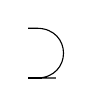
\begin{tikzpicture}[x=1pt,y=1pt,baseline=0pt]\draw (-3,12)--(\the\wd0,12) .. controls (\the\dimexpr\wd0+13pt\relax,12) and (\the\dimexpr\wd0+13pt\relax,-6) .. (\the\wd0,-6)--(7,-6);\draw (-3,-6)--(2,-6);\end{tikzpicture}}\box0\endgroup
\[
\Vert\quad G_{\lambda_\bullet}(\mathbb C_\bullet^i)
\]}
\[
F_{X_*}'(\mathbb C_*^\bullet)\simeq\mathbb C^\bullet(X_*)
=\text{complexe}\ \text{des cochaines non dégénérées sur }X_*
\]

\uline{Ex}
\[
X_* =\Delta_*^n,\qquad
\left\{\begin{aligned}
F_{\Delta_*^n}(M_*)&\simeq M_{[n]}\\
\mathbb C^\bullet(\Delta^n)&\simeq(\mathbb C_{[n]}^i)_i
=\Lambda^{*+1}k^{\Delta_{\mathrm{ens}}^n}
=(m\longmapsto k^{\operatorname{Mono}(\Delta_{\mathrm{ens}}^m,\Delta_{\mathrm{ens}}^n)})
\end{aligned}\right.
\]

On s'intéresse, pour $X_*$ fini, a
\[
[n]\longmapsto\operatorname{Hom}(F_{X_*},F_{\Delta_*^{\unsure{[n]|n}}})
\simeq\operatorname{Hom}(\underset{\substack{\Vert\\\lambda_\bullet^\vee}}{\mathbb C^\bullet(X_*)},
\underset{\substack{\Vert\\\Lambda^{*+1}k^{\Delta_{\unsure{\mathrm{ens}|\bullet}}^n}=\mathbb C_{[n]}^{\unsure{\bullet|\bullet\bullet}}}}{C^\bullet(\Delta_*^n)})
\]
\diagram{\begin{tikzcd}[column sep=large,row sep=large]
& \rotatebox{90}{$\simeq$} & {}\\
&\deleted{\operatorname{Hom}(G_{\lambda_*},G_{\underset{\substack{\Vert\\\mu_*}}{\underline{\mathbb C_{\unsure{n|*}}(\Delta^n)}}})} &\\
k[X_n]\arrow[uur,bend left=25] &
\operatorname{Hom}(\Delta^n,X_*)\simeq X_n \arrow[l] \arrow[uur] &
\end{tikzcd}}
\[
u\longrightarrow F(u)\qquad
\deleted{\lambda_*=\mathbb C_*[X]}
\]
\figure{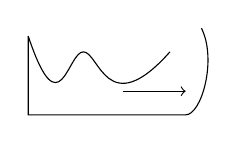
\begin{tikzpicture}
\draw (0,1) -- (0,0) -- (2,0) .. controls (2.2,0) and (2.4,.7) .. (2.2,1.1);
\draw (0,1) .. controls (.4,-.2) and (.5,.8) .. (.7,.8)
.. controls (.9,.8) and (1,-.1) .. (1.8,.8);
\draw[->] (1.2,.3) -- (2,.3);
\end{tikzpicture}}
\[
\deleted{\mathbb K\in\unsure{\mathrm{Ab}|\mathcal M}_k^*}
\]
\figure{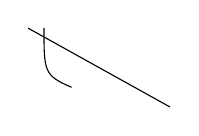
\begin{tikzpicture}\draw (0,1)--(1.8,0);\draw (.2,1) .. controls (.2,.45) and (.2,.4) .. (.55,.25);\end{tikzpicture}}
\[
\deleted{\operatorname{Hom}(}
\]

\margin{\[
\rotatebox{90}{$\simeq$}\qquad\unsure{\operatorname{Hom}_\bullet|\operatorname{Hom}}(\mathbb C_{\unsure{*\bullet|\bullet}}^{[n]},\lambda_\bullet^{\deleted{\unsure{[n]|*}}\vee\vee})
\]
\[
\rotatebox{90}{$\simeq$}\,!\qquad(\lambda_\bullet^{\vee\vee})_{[n]}=\lambda_{[n]}^{\vee\vee}
\]
\[
\Vert\qquad k[X_{[n]}]^{\vee\vee}
\]}

R. Ainsi \unsure{on|un} \unsure{a|ce} diagramme comm

\margin{\[
\deleted{\unsure{\operatorname{Hom}(\mathbb C_{\unsure{\bullet|*}}(X_*)^{\vee\vee},\Lambda^{\bullet+1}k^{\Delta^n})}}
\]
\[
\operatorname{Hom}_\bullet(\Lambda^{\bullet+1}k^{\Delta^n},\deleted{\unsure{\alpha|\mathbb C}}\mathbb C_\bullet(X_*)^{\vee\vee})
\]
\[
\rotatebox{90}{$\simeq$}\qquad\operatorname{Hom}(\mathbb C^\bullet(X_*),\Lambda^{\bullet+1}k^{\Delta^n})
\]
\[
\rotatebox{90}{$\simeq$}
\]}
\figure{\begin{tikzpicture}\draw (.5,1.4) .. controls (-.4,-.2) and (0,-.8) .. (.5,-.8) -- (1.6,-.8);\end{tikzpicture}}

\diagram{\begin{tikzcd}[column sep=large,row sep=large]
X_{[n]}\arrow[d] & \operatorname{Hom}(\Delta_*^n,X_*)\arrow[dd] \arrow[l,"\simeq" description,phantom]\\
k[X_{[n]}]\arrow[d,"(\text{iso si }X_n\text{ fini})"'] &\\
k[X_{[n]}]^{\vee\vee} &
\operatorname{Hom}(F_{\inserted{X_*}}\deleted{(X},F_{\Delta_*^n})\simeq\operatorname{Hom}(\mathbb C^\bullet(X_*),C^\bullet(\Delta_*^n))
\arrow[l,"\sim"']
\end{tikzcd}}

Faisons en particulier $X_*=\Delta_*^m$, on trouve donc
\diagram{\begin{tikzcd}[column sep=large,row sep=large]
\Delta_{[n]}^m=\operatorname{Hom}(\Delta^n,\Delta^m)\arrow[d]
\arrow[r,"\simeq" description,phantom] & \operatorname{Hom}(\Delta_*^n,\Delta_*^m)\arrow[d]\\
k(\Delta_{[n]}^m)\arrow[r,"\simeq" description,phantom] &
\operatorname{Hom}(F_{\Delta_*^m},F_{\Delta_*^n})\simeq
\end{tikzcd}}

\mspage{340}
